% This text is proprietary.
% It's a part of presentation made by myself.
% It may not used commercial.
% The noncommercial use such as private and study is free
% Sep. 2005 
% Author: Sascha Frank 
% University Freiburg 
% www.informatik.uni-freiburg.de/~frank/


\documentclass[hyperref={colorlinks=true,linkcolor=blue,urlcolor=blue},numbers]{beamer}
\usepackage{amsmath,paunits,shortcuts,overpic}
%\usepackage[usenames]{color}
\setbeamertemplate{navigation symbols}{}
\setbeamertemplate
    {footline}
    {\quad\strut\insertsection
      \hfill\insertframenumber/\inserttotalframenumber\strut\quad} 

\graphicspath{{./figs_wh/}}

\begin{document}
\graphicspath{{./figs_wh/}}

\section{Introduction}
\label{sec:introduction}

\begin{frame}
  \frametitle{Introduction}

This lecture -- look at Beer's law in a hydrostatic atmosphere

  \begin{itemize}

 \item We're only glancing over the  absorption line material on p. 129-130 for now, will come back to
it when we need absorption cross sections in particular satellite channels.

 \item Scattering: some nice examples of \href{http://www.met.reading.ac.uk/clouds/maxwell}{Light scattering by particles}

\item This time, introduce the complication of an absorbing gas with a vertically varying density

  \end{itemize}


\end{frame}


\begin{frame}
  \frametitle{Vertical absorption profile}
Focus p. 131 - 132, especially Fig. 4.23 and Fig. 4.24

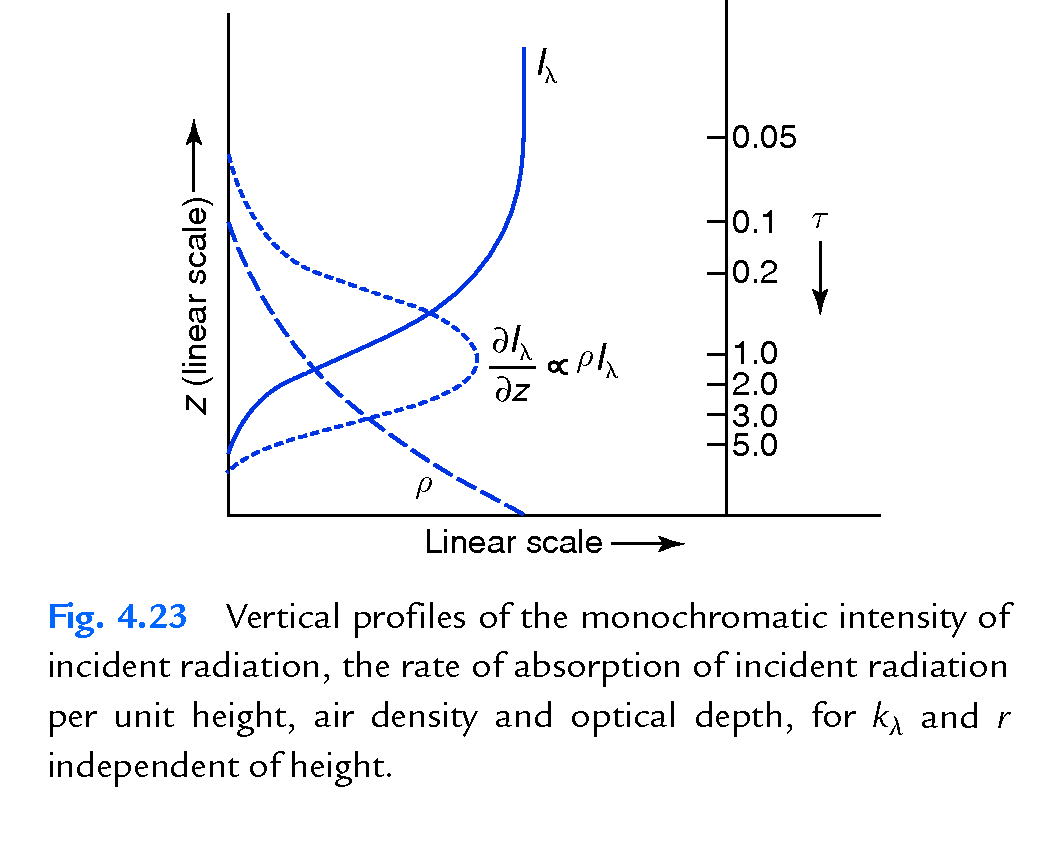
\includegraphics[width=0.6\textwidth]{vert_absorb.png}

Big question:  Why does the heating rate (i.e. the rate at which radiance is
building up in the atmosphere) peak at $\tau=1$

Reason we're interested:  It will also turn out that emission peaks at $\tau$=1,
which allows us to infer emission at different heights by measuring radiance at
different wavelengths

\end{frame}

\begin{frame}
  \frametitle{Review: Beers law for direct beam}

\begin{overpic}[tics=20,width=0.8\textwidth]{beers.png}
  \put(80,90){
     \begin{minipage}{0.4\textwidth}
         Define the ``slant path'' as $ds = dz/\cos \theta$
     \end{minipage}
   }
  \put(80,30){
     \begin{minipage}{0.4\textwidth}
         Note that in this case $z$ is positive downward!
     \end{minipage}
   }
\end{overpic}
 \end{frame}

\begin{frame}
  \frametitle{Absorption: Lorentz \& doppler line shapes}
\begin{overpic}[tics=20,width=0.6\textwidth]{lorentz.png}
  \put(100,60){
     \begin{minipage}{0.4\textwidth}
       \begin{itemize}
       \item The width of the lorentz line depends on collison frequency,
which is proportional to pressure.
\item The width of the doppler line depends on molecular speed, which is
proportional to $\sqrt{\text{temperature}}$
       \end{itemize}
     \end{minipage}
   }
\end{overpic}
\end{frame}

\begin{frame}
  \frametitle{Absorption lines are very narrow}
\begin{overpic}[tics=20,width=0.6\textwidth]{line_absorb.png}
  \put(60,60){
     \begin{minipage}{0.4\textwidth}
       \begin{itemize}
       \item Top figure goes from $\lambda=5.18\ \mum$ to
$\lambda=5.16\ \mum$
      \item Bottom figure goes from $\lambda=8.65\ \mum$ to
$\lambda=8.59\ \mum$
       \end{itemize}
But these lines are smooshed into wider bands by Doppler and Lorentz broadening
     \end{minipage}
   }
\end{overpic}
\end{frame}

\begin{frame}
  \frametitle{More review: }

  \begin{itemize}
  \item The slant  optical thickness (or slant optical depth)
is defined as:

\begin{equation*}
  d\sigma_\lambda = dTr = \frac{dF_\lambda }{F_\lambda} = -k_\lambda
  \rho_g ds
\end{equation*}
(where $k_\lambda$ is the mass absorption coefficient (\un{m^{2}\,kg^{-1}}))
\item In words, it's a measure of how ``thick'' a gas with density
$\rho_g$  is for photons with wavelength $\lambda$ in a layer of
thickness $ds$.

\item The ``vertical optical depth'' $d\tau_\lambda$ uses $dz$ instead of $ds$.
Since 
$dz = ds*\cos\theta$, the vertical optical depth is 
$d\tau_\lambda =\sigma_\lambda \cos \theta$

  \end{itemize}

\end{frame}

\begin{frame}
  \frametitle{What is $\rho_g?$   Start with: What is $\rho$?}

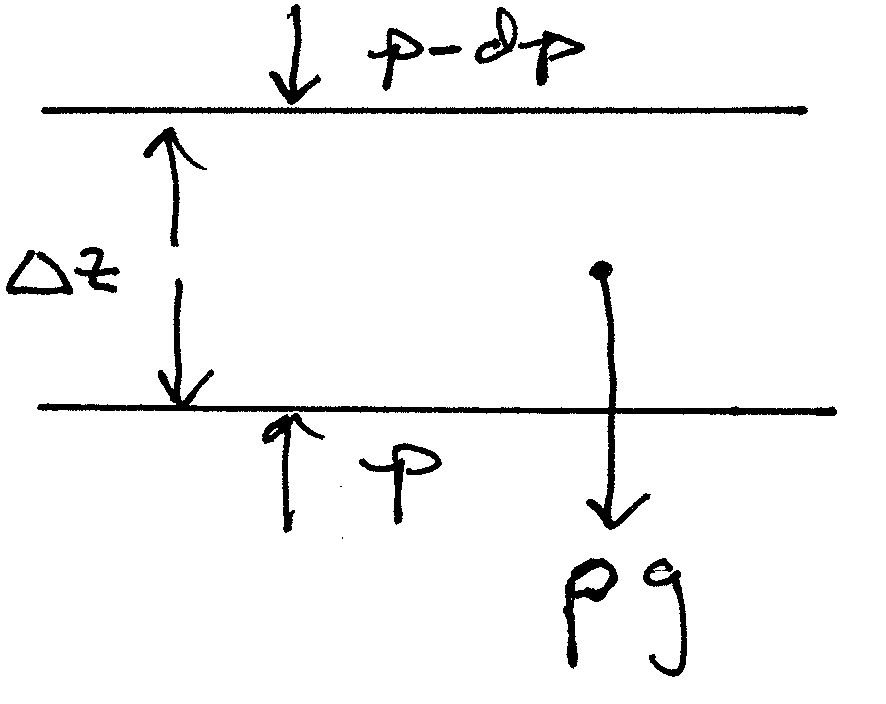
\includegraphics[width=0.4\textwidth]{hydrostat}

  \begin{itemize}


  \item Start with a layer with density $\rho_{air}$

  \item Assume hydrostatic balance for a layer of
thickness $\Delta z$, area $A$, volume $V=A \Delta z$


    \begin{itemize}
    \item Force down= ma = $\rho_{air} V g$ = $\rho_{air} A \Delta z g$
    \item pressure force up= dp A
    \item Balance requires $dp A = -\rho_{air} A \Delta z g$ or
    \item $dp = -\rho_{air} g dz$
    \end{itemize}
  \end{itemize}

\end{frame}

\begin{frame}
  \frametitle{Hydrostatic atmosphere, cont. (also see W\&H p. 67 }

  \begin{itemize}
  \item We want to integrate $dp^\prime = - \rho_{air} g dz^\prime$ from the surface to
a pressure level $p$.
\item Neglecting water vapor, the equation of state gives $p = \rho_{air} R_d T$
\item So use this.  Start from the surface with pressure = $p_0$, $z=0$, $\rho_{air}=\rho_0$
and integrate to height z, pressure p, density $\rho_{air}$

  \begin{gather*}
dp^\prime =-  \frac{ p}{R_d T} g dz^\prime \\
\int_{p_0}^p \frac{dp^\prime }{p^\prime} = - \int_0^z \frac{ g}{R_d T} dz^\prime = - \int_0^z \frac{ 1}{H} dz^\prime\\
\text{define the pressure scale height: $H_p$ as:}\\
\frac{1 }{H_p}  = \frac{ 1}{z}  \int_0^z \frac{ 1}{H} dz^\prime \\
\text{which leaves: } \int_{p_0}^p d \ln p^\prime  = - \frac{z }{H_p} 
  \end{gather*}
  \end{itemize}

\end{frame}

\begin{frame}
  \frametitle{Hydrostatic atmosphere, cont. }

  \begin{itemize}
  \item Finish the integration:

\begin{gather*}
 \int_{p_0}^p d \ln p^\prime  = - \frac{z }{H_p} \\
\ln \left ( \frac{ p}{p_0} \right ) = - \frac{z }{H_p} \\
p = p_0 exp \left (- \frac{z }{H_p} \right )
  \end{gather*}


\item and use the equation of state to get density:


  \begin{gather*}
 \rho_{air} R_d T = \rho_0 R_d T_0  exp \left (- \frac{z }{H_p} \right )\\
\rho_{air}  = \rho_0 \frac{ T_0}{T}  exp \left (- \frac{z }{H_p} \right ) \approx \rho_0 \exp \left (- \frac{z }{H_\rho} \right )
  \end{gather*}
where $H_\rho$ is the density scale height.  Typical values are $H_p$ = 10 km and $H_\rho$=8 km
  \end{itemize}

\end{frame}

\begin{frame}
  \frametitle{Finally, what is $\rho_g$?}

  \begin{itemize}
  \item If the gas is well mixed, then the mixing ratio:

    \begin{equation*}
      r_{g} = \frac{\text{kg gas} }{\text{kg air}} = \frac{ \rho_g}{\rho_{air}} = constant
    \end{equation*}

  \item Which means that

    \begin{equation*}
      \rho_g = r_{g} \rho_0 \exp \left (- \frac{z }{H_\rho} \right )
    \end{equation*}

  \item and so the vertical optical depth is:

    \begin{equation*}
      d\tau_\lambda = k_\lambda \rho_g dz = k_\lambda r_{g} \rho_0 \exp \left (- \frac{z }{H_\rho} \right ) dz
    \end{equation*}
  \end{itemize}
\end{frame}

\begin{frame}
  \frametitle{ now use $\rho_g$ to get $\tau_\lambda$}
  \begin{itemize}
  \item Integrate the optical thickness between some height $z^\prime =z$ 
and $\tau^\prime_\lambda = \tau_\lambda$ and the top of the atmosphere
where $z^\prime=\infty$ and $\tau^\prime_\lambda = 0$.  We need to introduce a minus sign
because we are moving downward (negative z direction) from the top:

\begin{gather*}
  \int_{\tau_\lambda}^0 d{\tau^\prime}_\lambda = -\int_z^\infty k_\lambda \rho_g dz^\prime = 
-\int_z^\infty k_\lambda r_{g} \rho_0 \exp \left (- \frac{z^\prime }{H_\rho} \right ) dz^\prime\\
0 - \tau_\lambda = H_\rho k_\lambda r_g \rho_0 \left [ 0 - \exp \left (- \frac{z }{H_\rho} \right ) \right ] \\
 \tau_\lambda = H_\rho k_\lambda r_g \rho_0 \exp \left (- \frac{z }{H_\rho} \right ) =
 H_\rho k_\lambda r_g \rho =  H_\rho \beta_a
  \end{gather*}
where $\beta_a = k_\lambda \rho_g =k_\lambda r_g \rho_{air}$ is the volume absorption coefficient.

\item So the vertical optical depth measured from the top of the atmosphere is proportional to the density
for a well-mixed absorber.




  \end{itemize}


\end{frame}

  \begin{frame}
    \frametitle{ Level of maximum heating from ozone absorption}

    \begin{itemize}
    \item The stratosphere is produced by solar heating due to ozone absorption of
ultraviolet photons.  

\item Recall the heating rate equation from (day 8, part II):

  \begin{equation*}
    \frac{ dT}{dt} = - \frac{1 }{\overline{\rho_{air}} c_p} \frac{ d F_N}{d z} 
  \end{equation*}
where $\Delta F_N$ is the net \textit{upward} flux.  


\item Since we know $\tau$, we know the direct beam flux from Beer's law (Lecture 8)

  \begin{equation*}
    F_\lambda = F_{\lambda 0} exp (- \tau_\lambda)
  \end{equation*}
and since $F_\lambda$ from the sun is downwards, and we are assuming no reflection,
$F_\lambda$ = $-F_N$ and $\frac{ dT}{dt}  \propto \frac{ dF_\lambda}{dz}$ 


\item So the heating rate will be maximum where $\frac{ d^2F_\lambda}{dz^2} = 0$

    \end{itemize}
  \end{frame}


  \begin{frame}
    \frametitle{heating rate: find $\tau$ where $\frac{ d^2F}{dz^2} = 0$  }

    \begin{itemize}
    \item since $F = F_0\exp(-\tau)$ and $\tau = C \exp(-z/H)$:
    \end{itemize}

      \begin{gather*}
        \frac{ dF}{dz} = -F_0 \frac{ d\tau}{dz} \exp(-\tau) = F_0 \frac{ C}{H} \exp(-z/H) \exp(-\tau) \\
\frac{ d^2F}{dz^2} = -\frac{ F C}{H^2}  \exp(-z/H) \exp(-\tau) +  \frac{ F C}{H}  \exp(-z/H) \exp(-\tau)\frac{d\tau }{dz}   = 0 \\
\frac{ 1}{H}  + \frac{ d \tau}{dz} =0 \\
\frac{1 }{H}  - \frac{C }{H}  \exp(-z/H) = 0 \\
\frac{1 }{H}  - \frac{ \tau}{H}  = 0 \\
\tau = 1
      \end{gather*}
      \begin{itemize}
      \item So the heating rate is maxium where $\tau=1$.
      \end{itemize}
  \end{frame}

\begin{frame}
  \frametitle{Vertical absorption profile for downward direct solar intensity}
\begin{overpic}[tics=20,width=0.7\textwidth]{vert_absorb.png}
  \put(80,60){
     \begin{minipage}{0.4\textwidth}
       \begin{itemize}
       \item Why does the direct beam change fastest at $\tau_\lambda
         = 1$?
       \item What height is this?
       \end{itemize}
     \end{minipage}
   }
\end{overpic}
\end{frame}

\begin{frame}
  \frametitle{ Beers law for ozone}

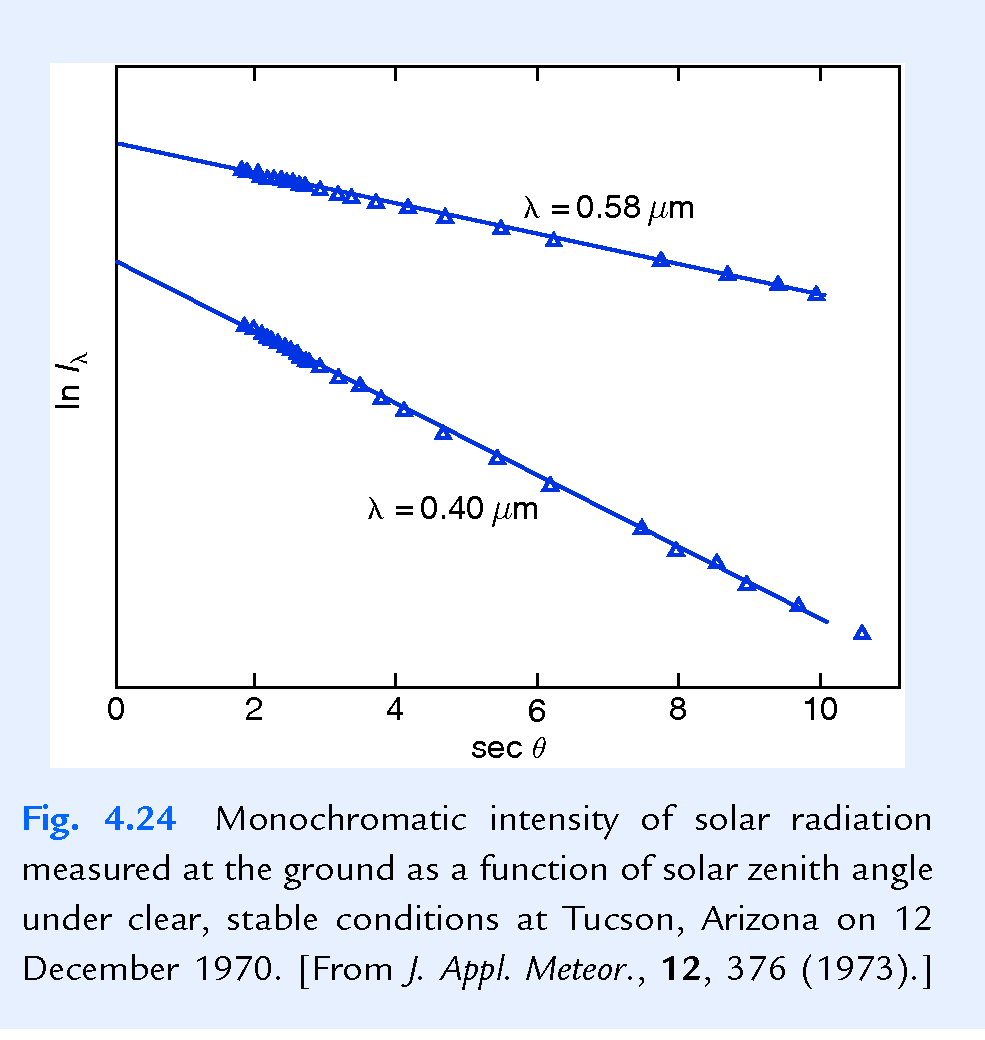
\includegraphics[width=0.8\textwidth]{beers_tucson.png}
\end{frame}

\begin{frame}
  \frametitle{Why are we getting straight lines of different slopes?}

  \begin{itemize}
  \item Beer's law:

    \begin{gather*}
      I_\lambda = I_{\lambda 0} \exp \left (  -\tau_\lambda /\cos \theta \right ) \\
\ln(I_\lambda) = \ln(I_{\lambda 0}) - \tau_\lambda /\cos \theta \\
\text{(assuming a plane parallel atmosphere})\\
    \end{gather*}


\item If $k_\lambda$ is constant:

  \begin{gather*}
\tau_\lambda = \int_z^\infty k_\lambda \rho_g dz^\prime    = k_\lambda \int_z^\infty \rho_g dz^\prime = k_\lambda \times Constant
  \end{gather*}


\item so the slope of the line is proportional to the mass absorption coefficient, which is strongest for ozone
in the ultraviolet (0.4 \mum)

  \end{itemize}

\end{frame}

\begin{frame}
  \frametitle{Discovery of the ozone hole }

  \begin{itemize}
  \item The ozone hole was discovered using land based 
\href{http://www.yesinc.com/products/data/spuv10/index.html}{sun photometers}
in 1985.

\item The hole was also detected by 
\href{http://www.nas.nasa.gov/About/Education/Ozone/history.html}{the TOMS instrument}


\item The cause wasn't fully understood until 
\href{http://ozonewatch.gsfc.nasa.gov/facts/history.html}{aircraft measurements} were made in
1987.


  \end{itemize}
\end{frame}

\begin{frame}
  \frametitle{Summary}

  \begin{itemize}
  \item Coverage: pp. 122-132 on scattering, absorption emission
  \item Main points:
    \begin{itemize}
    \item Scattering direction and efficience depends on wavelength $\lambda$ and particile size (r) via the size parameter
    \item Three distinct scattering regimes:  Rayleigh, Mie, Geometric
    \item Absorption depends on line strength and line width (function of temperature, pressure, wavelength)
    \item Vertical optical thickness relates the physical propoerties of absorbers/scatterers to driect beam transmission
    \end{itemize}
  \end{itemize}
\end{frame}



\end{document}
